\documentclass[12pt]{article}

\usepackage{sbc-template}
\usepackage{graphicx,url}
\usepackage[utf8]{inputenc}
\usepackage[T1]{fontenc}
\usepackage[brazil]{babel}
\usepackage{booktabs}
\usepackage{listings}

\lstset{
  basicstyle=\ttfamily\footnotesize,
  breaklines=true,
  frame=single,
  columns=fullflexible,
  keepspaces=true,
  literate={á}{{\'a}}1 {é}{{\'e}}1 {í}{{\'i}}1 {ó}{{\'o}}1 {ú}{{\'u}}1
           {ã}{{\~a}}1 {õ}{{\~o}}1 {ç}{{\c c}}1 {ê}{{\^e}}1 {â}{{\^a}}1
}

\sloppy

\title{Locadora de Veículos: Front-end integrado à API\\
(Trabalho Prático 2)}

\author{Geovanna Duarte}

\address{Curso de Análise e Desenvolvimento de Sistemas -- 4º semestre\\
  Disciplina: Tecnologias para Análise e Desenvolvimento de Sistemas\\
  Professor: Ramon Lacerda Marques
}

\begin{document}

\maketitle

\section{Descrição do problema}

Uma locadora de veículos precisa controlar sua frota, seus clientes e as locações em andamento. Sem um sistema, é difícil saber quais veículos estão disponíveis, quem está com qual carro, quando a devolução é esperada e quanto deve ser cobrado.

No Trabalho Prático 1 foram projetados o banco de dados e uma API REST que resolvem essa parte. Neste Trabalho Prático 2 foi construído o \textit{front-end} que consome essa API, permitindo operar a locadora pelo navegador: cadastrar, editar, excluir e pesquisar registros, abrir e encerrar locações e executar as consultas definidas na primeira etapa.

\section{Modelagem adotada}

O banco \texttt{LocadoraDb} (SQL Server) possui cinco entidades:

\begin{itemize}
  \item \textbf{Fabricante}: nome (único) e país de origem;
  \item \textbf{Categoria}: nome (único), descrição e valor de diária base (maior que zero);
  \item \textbf{Veículo}: modelo, ano, quilometragem, placa (única), cor e status (\textit{Disponível}, \textit{Alugado} ou \textit{Manutenção}); pertence a um Fabricante e a uma Categoria;
  \item \textbf{Cliente}: nome, CPF (único, 11 dígitos), e-mail (único) e telefone;
  \item \textbf{Aluguel}: liga um Cliente a um Veículo, com datas de retirada, devolução prevista e devolução, quilometragens inicial e final, valor da diária e valor total.
\end{itemize}

As relações são 1:N (Fabricante--Veículo, Categoria--Veículo, Cliente--Aluguel, Veículo--Aluguel). A exclusão em cascata foi evitada (\textit{Restrict}), e há restrições \textit{CHECK} para valores e datas. Um índice único filtrado impede dois aluguéis em aberto para o mesmo veículo. Os diagramas de classes e do banco estão na pasta \texttt{documentacao/} do repositório.

O back-end usa C\#, ASP.NET Core, Entity Framework Core e Swagger. Duas regras de negócio aparecem diretamente no front-end:
\begin{itemize}
  \item ao abrir um aluguel, o veículo passa para \textit{Alugado}; somente veículos \textit{Disponíveis} podem ser alugados;
  \item ao registrar a devolução, o valor total é calculado como número de dias $\times$ valor da diária (mínimo de um dia), a quilometragem do veículo é atualizada e ele volta a \textit{Disponível}.
\end{itemize}

\section{Rotas da API utilizadas}

Todas as rotas têm o prefixo \texttt{/api}. A Tabela~\ref{tab:rotas} resume as rotas consumidas pelo front-end.

\begin{table}[ht]
\centering
\small
\begin{tabular}{@{}lll@{}}
\toprule
\textbf{Recurso} & \textbf{Método e rota} & \textbf{Uso no front-end}\\
\midrule
Fabricantes, Categorias, Clientes & GET/POST/PUT/DELETE & CRUD completo\\
Veículos & GET/POST/PUT/DELETE & CRUD completo\\
Aluguéis & GET/POST/PUT/DELETE & abrir, editar, listar, excluir\\
\midrule
Veículos & GET \texttt{/veiculos/disponiveis} & consulta (categoria opcional)\\
Veículos & GET \texttt{/veiculos/por-fabricante/\{id\}} & consulta por fabricante\\
Clientes & GET \texttt{/clientes/\{id\}/historico} & histórico do cliente\\
Aluguéis & GET \texttt{/alugueis/em-aberto} & consulta de abertos\\
Aluguéis & GET \texttt{/alugueis/por-periodo} & consulta por período\\
Aluguéis & PUT \texttt{/alugueis/\{id\}/devolucao} & registrar devolução\\
\bottomrule
\end{tabular}
\caption{Rotas da API consumidas pelo front-end.}
\label{tab:rotas}
\end{table}

\subsection{Consultas ao banco}

As cinco consultas do Trabalho Prático 1 usam dois tipos de junção. Duas delas, com resultado visto no front-end, são detalhadas a seguir.

\paragraph{Veículos disponíveis por categoria (\textit{LEFT JOIN}).} A rota usa \texttt{Include()} do Entity Framework, que gera um \textit{LEFT JOIN} com Fabricantes e Categorias.

\begin{lstlisting}[language={[Sharp]C}]
_context.Veiculos
  .Include(v => v.Fabricante)
  .Include(v => v.Categoria)
  .Where(v => v.Status == StatusVeiculo.Disponivel);
// + .Where(v => v.CategoriaId == categoriaId) se informado
\end{lstlisting}

\paragraph{Aluguéis por período (\textit{INNER JOIN}).} A rota usa \texttt{join} explícito do LINQ entre Aluguéis, Clientes e Veículos, filtrando pela data de retirada.

\begin{lstlisting}[language={[Sharp]C}]
from a in _context.Alugueis
join c in _context.Clientes on a.ClienteId equals c.Id
join v in _context.Veiculos on a.VeiculoId equals v.Id
where a.DataRetirada >= inicio && a.DataRetirada <= fim
orderby a.DataRetirada
select new AluguelResponseDto { ... }
\end{lstlisting}

As demais consultas são: veículos por fabricante (\textit{INNER JOIN}), aluguéis em aberto (\textit{LEFT JOIN}) e histórico de aluguéis do cliente (\textit{LEFT JOIN}).

\section{Wireframes}

Os wireframes de média fidelidade, que guiaram a criação das telas, estão disponíveis no Figma:

\begin{center}
\url{https://www.figma.com/design/Pz6ScsLEmc0BYXTxuMihyh}
\end{center}

\section{Implementação do front-end}

O front-end fica na pasta \texttt{frontend/} do repositório, na mesma estrutura do Trabalho Prático 1. Foi desenvolvido com React, Vite e Bootstrap (JavaScript, HTML e CSS), e se comunica com a API por requisições \texttt{fetch}, concentradas em um único arquivo (\texttt{api.js}). O CORS foi habilitado no back-end para a origem \texttt{http://localhost:5173}.

Para evitar repetição, cada entidade é descrita em um arquivo de configuração (\texttt{config.js}), que define rota, campos do formulário, colunas da tabela, filtros e consultas. Um único componente genérico (\texttt{Crud.jsx}) lê essa configuração e entrega, para qualquer entidade:
\begin{itemize}
  \item listagem em tabela com botões \textbf{Editar} e \textbf{Excluir};
  \item formulário de cadastro e de edição em janela modal, com campos obrigatórios e listas de seleção para chaves estrangeiras (por exemplo, fabricante e categoria em Veículos);
  \item filtros personalizados em pelo menos dois campos por entidade (aplicados no navegador sobre os registros carregados da API);
  \item um seletor de \textbf{consulta no banco}, que chama as rotas especiais da API;
  \item exibição das mensagens de erro devolvidas pela API (por exemplo, exclusão bloqueada por existirem registros relacionados ou CPF duplicado).
\end{itemize}

Os dados exibidos vêm sempre do banco, por meio da API; não há dados estáticos nem simulados no front-end.

\section{Telas desenvolvidas}

A navegação principal contém: Painel, Veículos, Fabricantes, Categorias, Clientes e Aluguéis. A Tabela~\ref{tab:telas} resume as funcionalidades de cada tela.

\begin{table}[ht]
\centering
\small
\begin{tabular}{@{}p{2.2cm}p{4.3cm}p{6.5cm}@{}}
\toprule
\textbf{Tela} & \textbf{Filtros de pesquisa} & \textbf{Consultas ao banco (rotas)}\\
\midrule
Veículos & modelo, placa, fabricante, status & disponíveis por categoria; por fabricante\\
Fabricantes & nome, país & ---\\
Categorias & nome, descrição & ---\\
Clientes & nome, CPF, e-mail & histórico de aluguéis do cliente\\
Aluguéis & cliente, placa, veículo & em aberto; por período de retirada\\
\bottomrule
\end{tabular}
\caption{Filtros e consultas por tela. Todas têm cadastro, edição e exclusão; em Aluguéis, a edição vale só para locações em aberto e há o botão \textit{Devolução}.}
\label{tab:telas}
\end{table}

\subsection{Painel}

O painel inicial (Figura~\ref{fig:painel}) mostra indicadores obtidos da API (veículos na frota, disponíveis agora, clientes e aluguéis em aberto) e a lista de devoluções pendentes, ordenada da mais próxima para a mais distante.

\begin{figure}[ht]
\centering
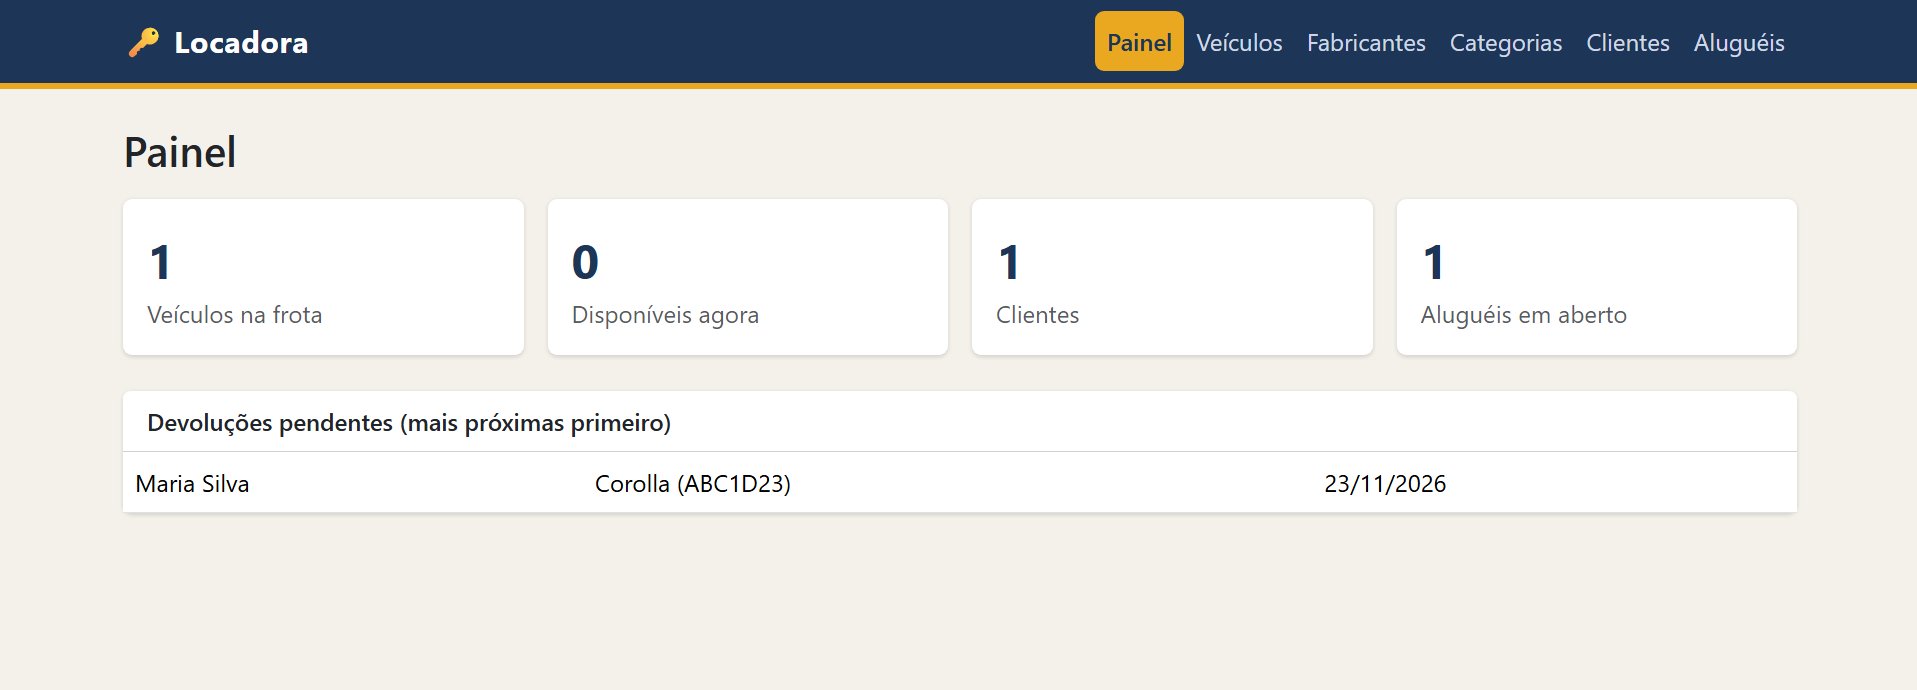
\includegraphics[width=\textwidth]{figs/painel.png}
\caption{Painel com indicadores e devoluções pendentes.}
\label{fig:painel}
\end{figure}

\subsection{Cadastros: Fabricantes e Categorias}

As telas de Fabricantes (Figura~\ref{fig:fab}) e Categorias (Figura~\ref{fig:cat}) seguem o padrão de listagem com filtros por dois campos, botão \textbf{+ Novo} e ações de editar e excluir. Em Fabricantes, a coluna \textit{Veículos} mostra a quantidade de veículos ligados a cada fabricante.

\begin{figure}[ht]
\centering
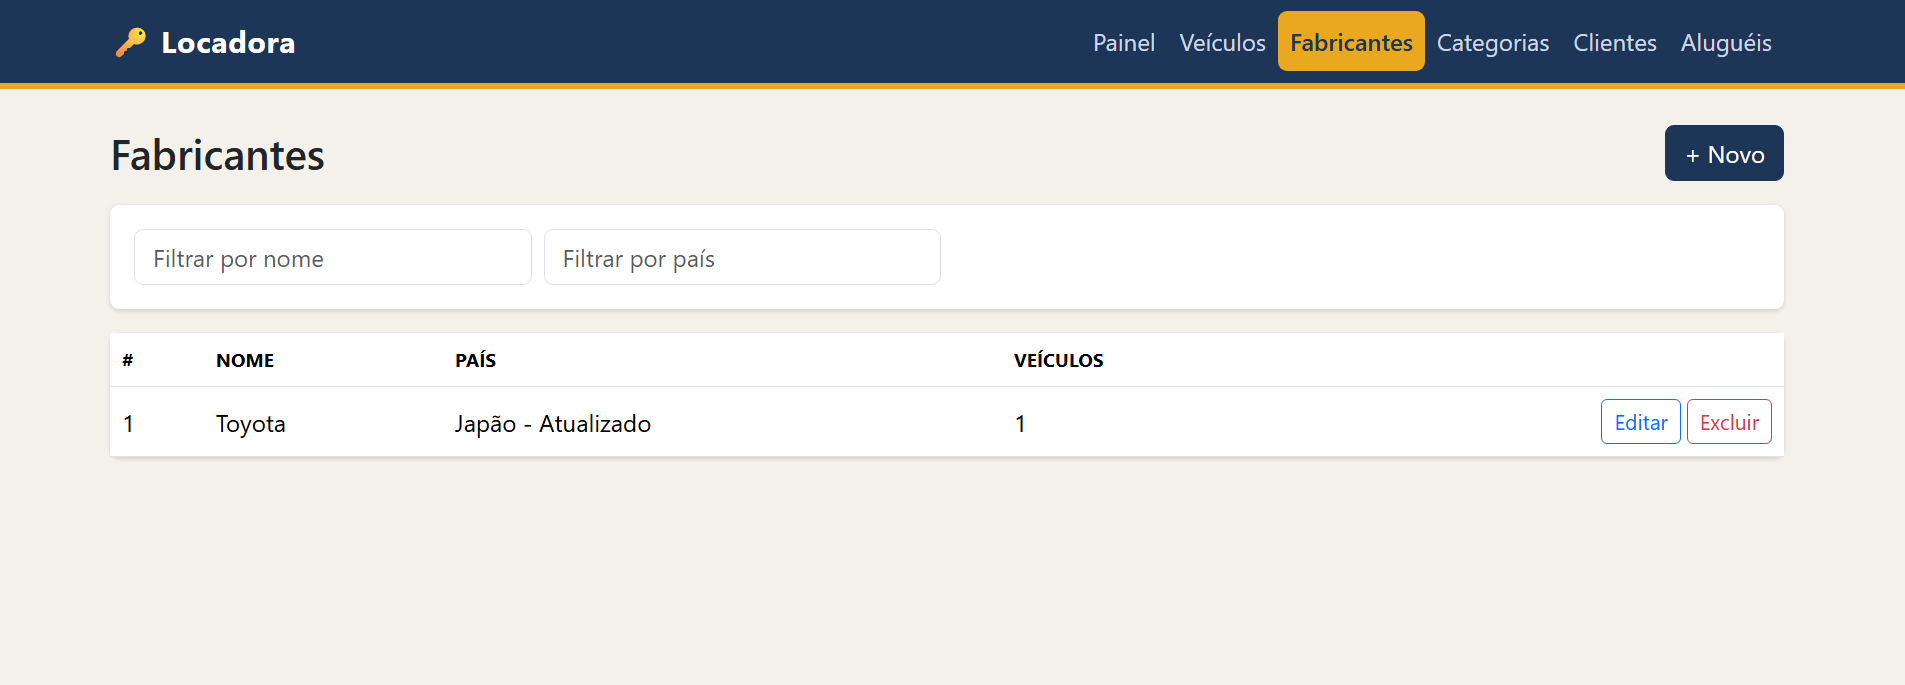
\includegraphics[width=\textwidth]{figs/fabricantes.png}
\caption{Tela de Fabricantes, com filtros por nome e país.}
\label{fig:fab}
\end{figure}

\begin{figure}[ht]
\centering
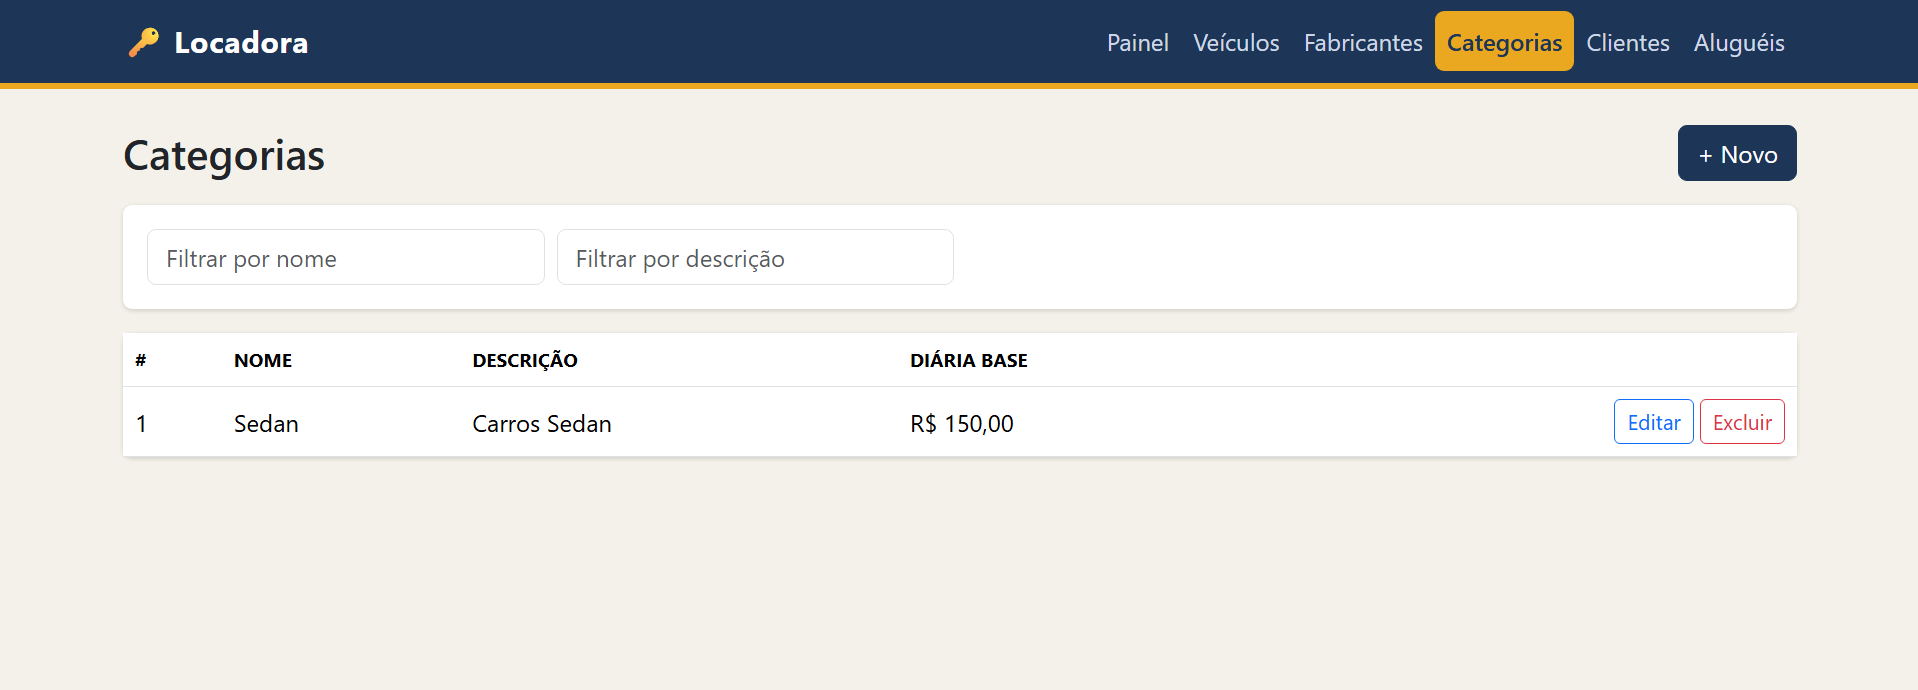
\includegraphics[width=\textwidth]{figs/categorias.png}
\caption{Tela de Categorias, com filtros por nome e descrição.}
\label{fig:cat}
\end{figure}

\subsection{Veículos}

A tela de Veículos (Figura~\ref{fig:veic}) apresenta o status com cores (verde para disponível) e filtros por modelo, placa, fabricante e status. No bloco \textit{Consulta no banco}, o usuário escolhe entre \textit{Veículos disponíveis (por categoria)}, que chama \texttt{GET /api/veiculos/disponiveis}, e \textit{Veículos por fabricante}, que chama \texttt{GET /api/veiculos/por-fabricante/\{id\}}. O botão \textit{Limpar} volta à listagem completa.

\begin{figure}[ht]
\centering
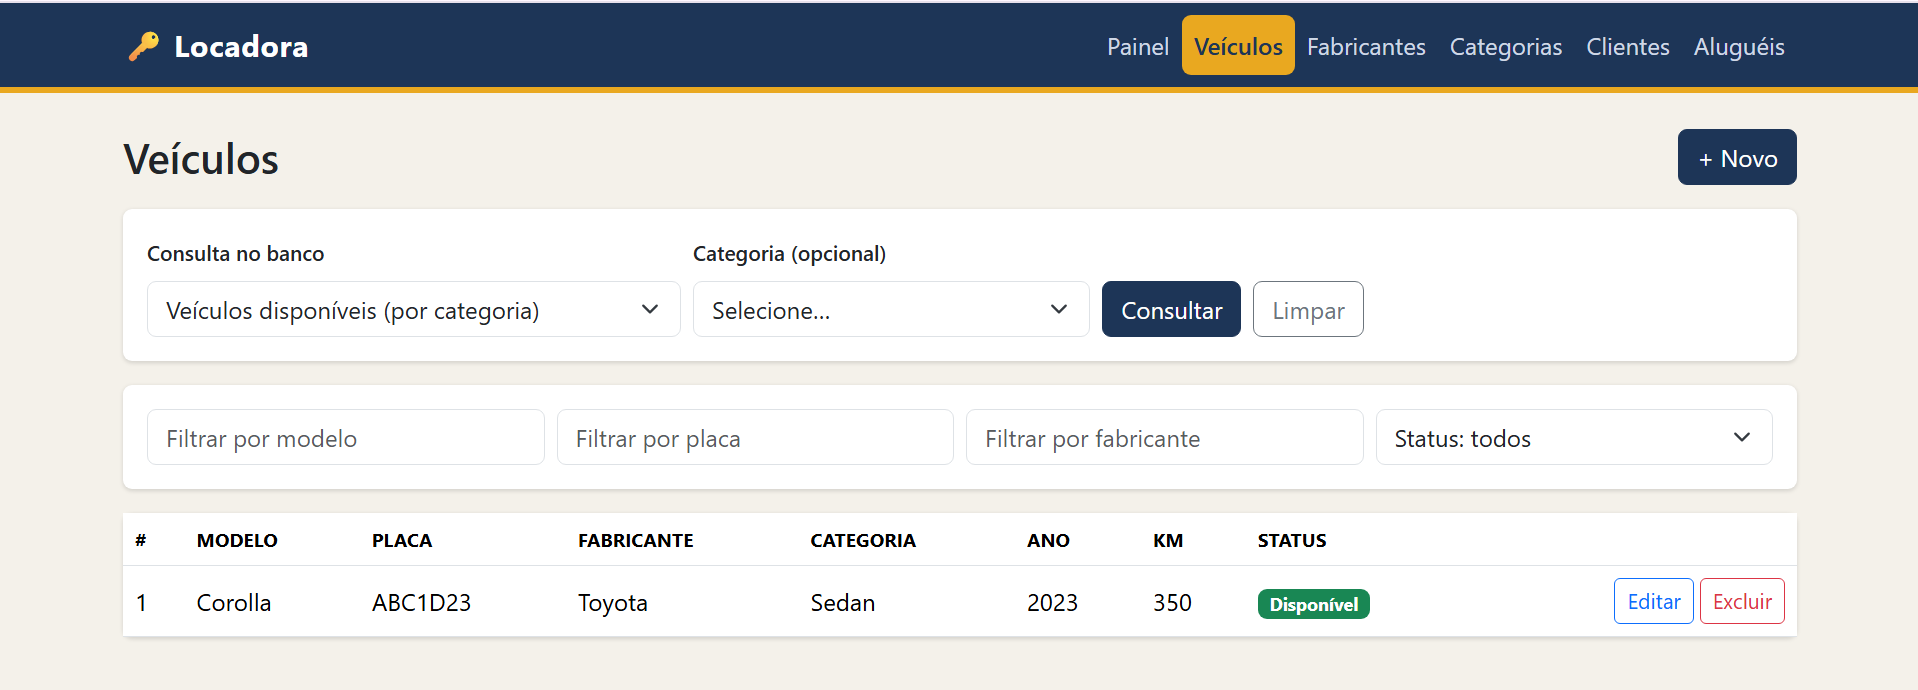
\includegraphics[width=\textwidth]{figs/veiculos.png}
\caption{Tela de Veículos com consulta ao banco e filtros.}
\label{fig:veic}
\end{figure}

\subsection{Clientes}

Em Clientes (Figura~\ref{fig:cli}), além do CRUD e dos filtros por nome, CPF e e-mail, a consulta \textit{Histórico de aluguéis do cliente} pede a escolha de um cliente e chama \texttt{GET /api/clientes/\{id\}/historico}, exibindo as locações dele em ordem da mais recente para a mais antiga.

\begin{figure}[ht]
\centering
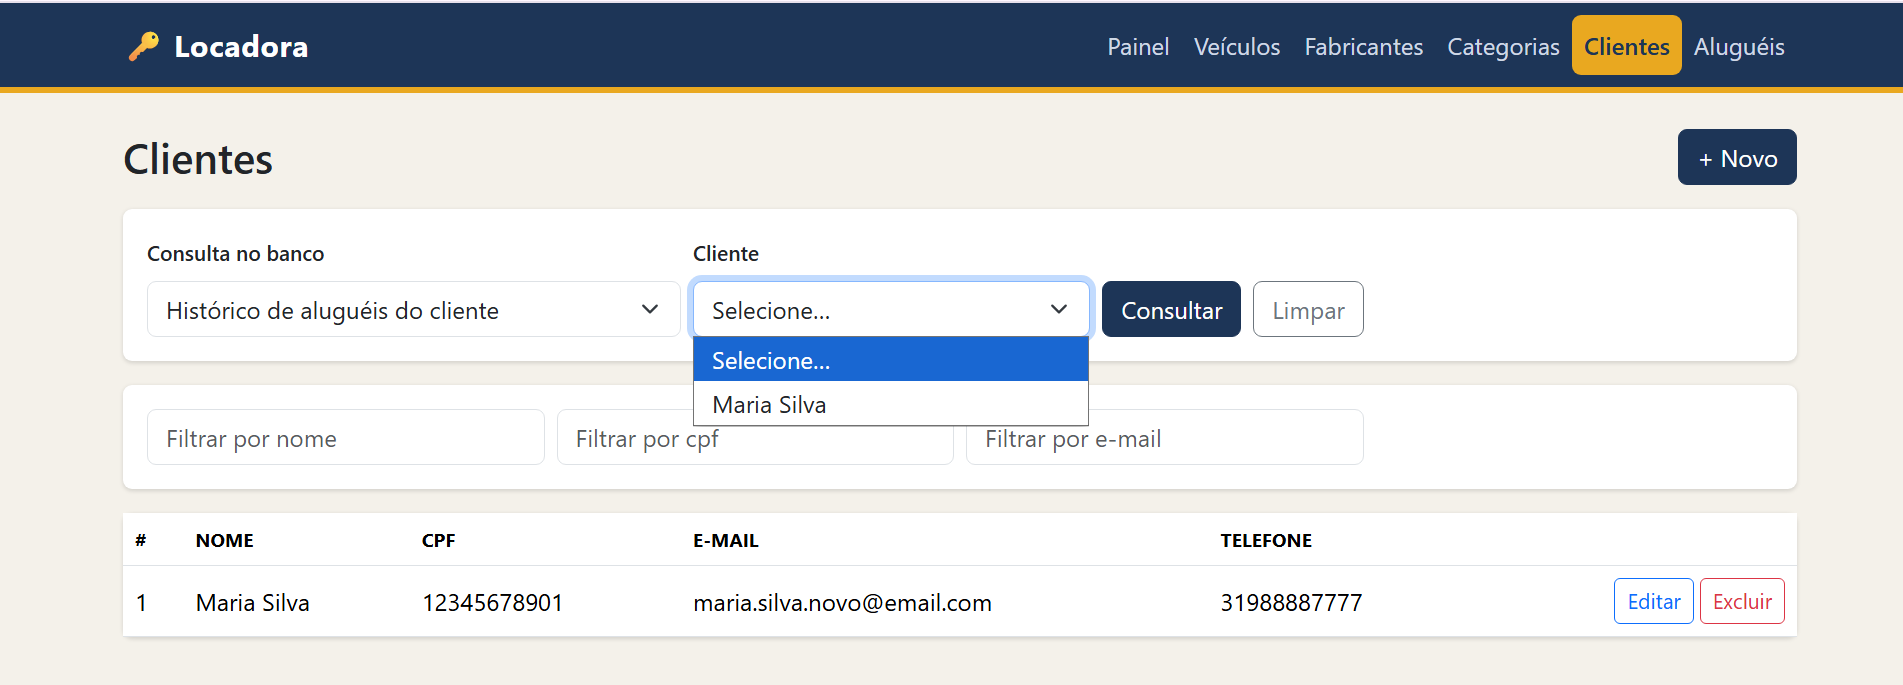
\includegraphics[width=\textwidth]{figs/clientes.png}
\caption{Tela de Clientes com a consulta de histórico (seleção do cliente).}
\label{fig:cli}
\end{figure}

\subsection{Aluguéis}

A tela de Aluguéis (Figura~\ref{fig:alu}) é a que concentra o fluxo principal da locadora. Ao criar um aluguel, apenas veículos disponíveis aparecem na lista de seleção (rota \texttt{/veiculos/disponiveis}). Para locações em aberto, a coluna de ações mostra \textbf{Devolução}, \textbf{Editar} e \textbf{Excluir}; ao registrar a devolução, informam-se data e quilometragem final, e a API calcula o total. As consultas disponíveis são \textit{Aluguéis em aberto} (\texttt{GET /api/alugueis/em-aberto}) e \textit{Aluguéis por período} (\texttt{GET /api/alugueis/por-periodo}).

\begin{figure}[ht]
\centering
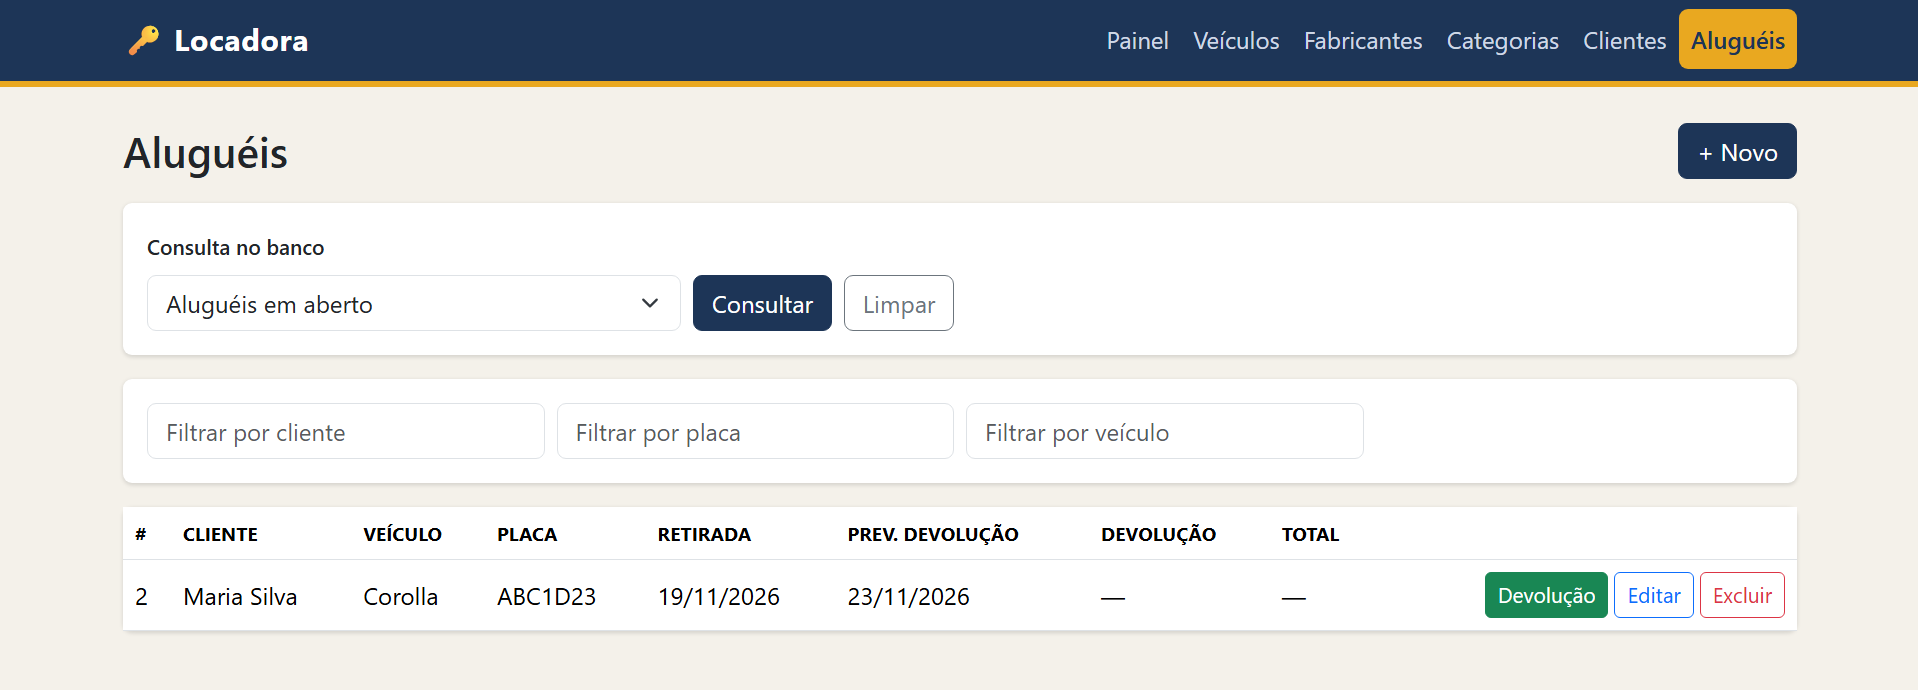
\includegraphics[width=\textwidth]{figs/alugueis.png}
\caption{Tela de Aluguéis exibindo o resultado da consulta de aluguéis em aberto.}
\label{fig:alu}
\end{figure}

\section{Como executar}

\begin{enumerate}
  \item Back-end: configurar a \textit{connection string} em \texttt{appsettings.json}, executar \texttt{dotnet ef database update} e \texttt{dotnet run} (porta 5273; Swagger em \texttt{/swagger});
  \item Front-end: \texttt{cd frontend}, \texttt{npm install} e \texttt{npm run dev}, acessando \texttt{http://localhost:5173}. Se a API estiver em outra porta, ajustar \texttt{VITE\_API\_URL} no arquivo \texttt{.env}.
\end{enumerate}

\section{Entregáveis}

\begin{itemize}
  \item Repositório GitHub: \url{https://github.com/Geovanna-dev/locadora-veiculos}
  \item Wireframes (Figma): \url{https://www.figma.com/design/Pz6ScsLEmc0BYXTxuMihyh}
  \item Vídeo de apresentação (3 a 5 minutos): enviado na atividade do Canvas.
\end{itemize}

\end{document}

